 \documentclass[11pt]{article}

\usepackage{amsmath}
\usepackage{amsxtra}
\usepackage{amsfonts}
\usepackage{amssymb}
\usepackage{amsthm}
\usepackage{graphicx}
\usepackage{mathtools}
\usepackage{dsfont}
\usepackage{hyperref}

\graphicspath{ {/Users/andrew/hw/math191k/figures/}}

\usepackage[margin=3cm]{geometry}
\newcommand{\eps}{\varepsilon}
\newcommand{\Z}{\mathbb{Z}}
\newcommand{\N}{\mathbb{N}}
\newcommand{\R}{\mathbb{R}}
\newcommand{\Q}{\mathbb{Q}}
\newcommand{\W}{\mathcal{W}}
\newcommand{\U}{\mathcal{U}}
\newcommand{\V}{\mathcal{V}}
\newcommand{\C}{\mathbb{C}}
\newcommand{\K}{\mathcal{K}}

\newcommand{\set}[1]{\{ #1 \}}
\newcommand{\gen}[1]{\left\langle #1 \right\rangle}
\newcommand{\floor}[1]{\left\lfloor #1 \right\rfloor}
\newcommand{\abs}[1]{\left| #1 \right|}
\renewcommand{\phi}{\varphi}
\renewcommand{\Re}{\operatorname{Re}}
\renewcommand{\Im}{\operatorname{Im}}
\newcommand{\conj}[1]{\mkern 1.5mu\overline{\mkern-1.5mu#1\mkern-1.5mu}\mkern 1.5mu}
\newcommand{\defeq}{\vcentcolon=}
\newcommand{\identity}{\mathds{1}}

\DeclareMathOperator{\im}{im}
\DeclareMathOperator{\res}{Res}
\DeclareMathOperator{\Arg}{Arg}
\DeclareMathOperator{\parg}{arg}
\DeclareMathOperator{\Log}{Log}

\theoremstyle{plain}
\newtheorem{thm}{Theorem}

\theoremstyle{definition}
\newtheorem{recall}{Recall}
\newtheorem{remark}{Remark}
\newtheorem{definition}{Definition}
\newtheorem{prop}{Proposition}
\newtheorem{cor}{Corollary}
\newtheorem{lemma}{Lemma}
\newtheorem{ex}{Example}
\newtheorem{claim}{Claim}
\newtheorem{exercise}{Exercise}
\newtheorem{notation}{Notation}
\newtheorem{question}{Question}

\title{Lectures notes on knot theory}
\author{Andrew Berger}

\begin{document}
\maketitle

\clearpage

\tableofcontents


\clearpage
\section{Disclaimer}

Caution - these lecture notes have not been proofread and may contain errors, due to either the lecturer or the scribe. Please send any corrections or suggestions to \href{mailto:andbberger@berkeley.edu}{andbberger@berkeley.edu}

\clearpage

\section{1/19/16: Introduction + Motivation}

Start with a joke: ``Applied Math majors may have misread the course title''

\bigskip
- hand out syllabus \& table of knots

- administration \& logistics

- ``idea'' of class structure

- find out about class (their backgrounds \& interests)

\bigskip
- introduce some material:

1) knots come from real life: tie ends of string together

- unknots

- simplest possible knot = trefoil

2) not everything is a circle

- want to distinguish them

- knot complements

- techniques?

3) links ? can be complicated while component knots simple

4) crossings / deformations

- swap crossings of trefoil to get its mirror (interesting fact: they're not equivalent!)

5) usefulness:

- want to know when objects are knotted

- get all 3-dimensional spaces

- applications to physics

\clearpage
\section{1/21/16: 2nd class}

\subsection{Logistical things}

Talk to Chris if you're uncomfortable with group theory. There are going to be two projects (long and short) - we'll start breaking up in to groups to work on those starting the second week of February.

\subsection{Minimal introduction to point-set topology}

Just to set terms and notation for future reference.


\begin{definition}
  Some miscellaneous definitions:

  \begin{itemize}
  \item $\R^n \defeq \R \oplus \ldots \oplus \R$
  \item $B^n = \set{x \in \R^n | \abs{x} \leq 1}$ note that in general this includes the boundary (which we call $\partial B^n = S^{n -1}$, the $(n - 1)$-sphere)
  \item There are many ways to get the inclusion $\R^m \subseteq \R^n$ for $m \leq n$, as a convention just take the first $m$ elements from $\R^n$
  \end{itemize}
\end{definition}


\begin{remark}
  The (closed) line and circle are the only 1-dimensional topological spaces (once we have defined appropriate notions of equivalence). More on this later
\end{remark}


\begin{definition}[Homeomorphism]

  We say that $f$ is a \emph{homeomorphism} if it is a bicontinuous bijection (both $f$ and its inverse are continuous). Two topological spaces $X, Y$ are homeomorphic
  if there exists $f: X \to Y$ a homeomorphism, denoted $X \cong Y$
\end{definition}

\begin{remark}
  Given $X, Y$ topological spaces and $f: X \to Y$ a homeomorphism we can `pull' the notion of openness in $X$ into
  a notion of openess in $Y$: $A \subseteq Y$ is open if $f^{-1}(A)$ is open in $X$
\end{remark}



\begin{ex}
  Examples of homeomorphisms
  \begin{itemize}
  \item $(0, 1) \cong \R$. As an exercise find the homeomorphism that is witness to this fact (hint: use an arctangent)
  \item A square in the plane is homeomorphic to a circle in the plane
  \item $\R^n \not \cong \R^m$ for $n \neq m$: dimension is invariant under homeomorphism. This is a deep result
    that is supposed to be hard to prove
  \end{itemize}
\end{ex}


\begin{definition}[Knot]
  A knot is a one-dimensional subset of $\R^3$ that is homeomorphic to $S^1$.

  We can specify a knot $K$ by specifying an embedding (smooth injective) $f: S^1 \to R^3$
  so that $K = f(S^1)$. For $f$ to be smooth, all of its derivatives must exist.
\end{definition}


\begin{ex}
  Examples of embeddings specifying knots
  \begin{itemize}
  \item $f = \mathds{1}$ (abuse of notation here) specifies a circle
  \item The infinite non-knot example we looked at yesterday fails to be a knot because the derivative does not exist
    at the limit point
  \end{itemize}
\end{ex}


\begin{definition}[Link]
  Given a collection of knots $\set{K_i}$, we define a link $L = \bigcup_i K_i$ (disjoint union)
\end{definition}

The study of links is different from the study of knots, due to ``linking behavior''. Roughly speaking: knots can be very complicated as well their disjoint unions, but moreover, links can get very complicated while their connected components may all be unknots.

\subsection{Equivalence of knots}

Our word for equivalence of knots is ambient isotopy. This refers to the fact that the homeomorphism that is witness
to the equivalence of the knots acts on the ambient space the knots lives and not only on the knot itself.




\begin{definition}[Equivalence of knots]
  For $K_1, K_2$ knots, we say that $K_1 \cong_{isotopic} K_2$
  if there exists a (orientation-preserving) homeomorphism $f: \R^3 \to \R^3$ such that $f(K_1) = K_2$.

  More precisely we require that there exists a 1-parameter family $\set{f_t}_{0 \leq t \leq 1}$ of smooth homeomorphisms such that $f_0 = \identity$ and $f_1 = f$. In particular, we cannot have an isotopy that shrinks a knot to a point.

  This aligns pleasingly for the intuitive notion that knots are equal when they can be deformed to each other:
  $f$ here is just the global deformation.
\end{definition}

\begin{remark}
  Careful about the notation here: $K_1 \cong K_2 \cong S^1$ holds for any knots $K_1, K_2$
\end{remark}


\begin{definition}[Knotted]
  We say that a knot $K$ is \emph{knotted} if $K \not \cong_{isotopic} S^1$
\end{definition}


\begin{definition}[Planar diagram of $K$]
  When we visualize knots we make some projection $\R^3 \to \R^2$ (with defined coordinate system). The na\"ive projection that discards information about the crossings
  is called the universe and is not necessarily unique. The planar diagram is this projection with crossing information captured.

\end{definition}

\begin{ex}
Examples of invariants (under equivaence)
\begin{itemize}
  \item Dimension is an invariant of isotopy
  \item The crossing number is the minimal number of crossings in a given diagram
\end{itemize}
\end{ex}

\subsection{Reidemeister moves}

What does an isotopy mean for planar diagrams? The famous Reidemeister moves


\begin{definition}[Reidemeister moves]

  \begin{enumerate} Refer to figure~\ref{fig:reidemeister}
  \item R0: You can straighten wiggly lines
  \item R1: You can undo twists
  \item R2: You can seperate underpasses (that don't intersect)
  \item R3: You can move a line behind an intersection across the intersection
  \end{enumerate}
\end{definition}


\begin{figure}[h]
  \centering
  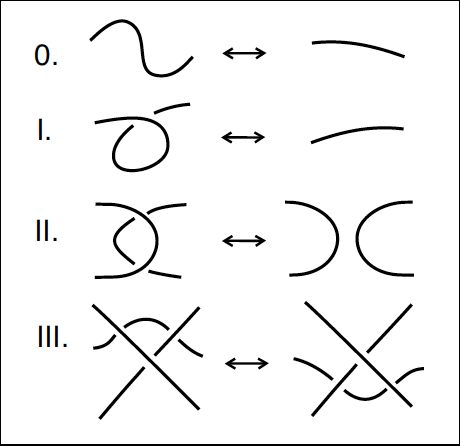
\includegraphics[width=\textwidth]{reidemeister.png}
  \caption{Sketch of allowed Reidemeister moves}\label{fig:reidemeister}
\end{figure}


\begin{thm}
$K_1 \cong_{isotopic} K_2$ iff their diagrams can be obtained from each other using the Reidemeister moves
\end{thm}

Wherein Chris struggles to draw a trefoil.

\begin{exercise}
  \begin{enumerate}
    \item Show that the figure eight knot is equivalent to its mirror.
    \item Take your favorite knot diagram and show that it is equivalent to the diagram obtained as follows: Take an arc on the left-most side of your diagram, put a twist in it and then pull it all over to the right side of the diagram. (The point of this exercise is to give an abstract proof of equivalence using Reidemeister moves without worrying about the explicit diagram.)
    \item Show that an unknot with a couple of loops is equivalent to the unknot \emph{without} using R1
  \end{enumerate}
\end{exercise}


\clearpage
\section{1/26/16: recap of the last lecture}

\subsection{Recap of last lecture}

What does it mean to be a knot? To be knotted?


\begin{recall}
  Recall that a knot $K$ is a subset of $\R^3$ that is homeomorphic to $S^1$.

  We could equally as well have defined a knot to be the image $f(S^1)$ of a smooth embedding $f: S^1 \to \R^3$.
\end{recall}


\begin{notation}
  Let's fix our notation for ambient isotopy (the kind that captures a notion of knottedness) and homeomorphism (under which all knots are equivalent), being very careful to distinguish between them.
  \begin{itemize}
  \item For $K_1, K_2$ knots that are equivalently knotted (or isotopic) and write $K_1 \cong K_2$
  \item We write homeomorphism with $\approx$. For instance, all knots $K$ are homeomorphic to $S^1$, $K \approx S^1$
  \end{itemize}
\end{notation}

\subsection{Intro to knot complement}

We expect that the knot complement $\R^3 \setminus K$ should somehow capture the notion of knottedness. Can we formalize that?

`It's not the space itself - it's what the knot is doing in 3-dimensional space that matters, and this theorem captures that precisely'


\begin{thm}[Gordon-Luecke]
  If $\R^3 \setminus K_1 \approx \R^3 \setminus K_2$ then $K_1 \cong K_2$
\end{thm}


\begin{remark}
  The fundamental group sometimes allows us to answer the question `$\R^3 \setminus K_1 \approx \R^3 \setminus K_2$?' and therefore turn this into an algebraic problem.

  Francesca pointed out that the converse of the preceding theorem is easily proved, directly from the definition of equivalence. Do it as an exercise!
\end{remark}

\begin{question}
  Marissa asked: when is a knot equal to its mirror? Chris isn't aware of any general classification results - maybe when the Jones polynomial has palyndromic coefficients.
  Another question: if $K_1 \cong K_2$ is it true that $K_1^\ast \cong K_2^\ast$ (here $K^\ast$ indicates the knot mirror)
  Yet another question: if $K_1 \cong K_2$ and $K_1 \cong K_1^\ast$ is it true that $K_2 \cong K_2^\ast$? Someone
  pointed out that if you can prove the previous statement, then this statement is easily proved to be true.
\end{question}

\subsection{Hard Unknots}

Chris struggles again to draw a trefoil.

Let's fix a notion of complexity for knot diagrams - we say that the complexity of a diagram is the crossing number of that diagram.

Recall that a knot is equivalent to the unknot if it \emph{has a diagram} with crossing number zero. A natural direction to head in towards proving that the trefoil is not the unknot might be to show that any Reidemiester move can
not decrease the complexity of the trefoil diagram - but one needs to be very careful here as there may be a sequence that increases in complexity for a while before decreasing.

This motivates the concept of hard unknots: unknots that require a sequence of Reidemeister moves increasing the complexity of the diagram before the complexity finally falls to zero.


To begin with let's study a hard unknot called `the culprit' from the paper \emph{Hard Unknots and Collapsing Tangles} (Kauffman, Lambropoulou). Can you see how to untangle this knot?

\clearpage
\section{1/28/16}

Agenda: what sort of invariants; solved problem from last class;
oriented knots, linking numbers, fundamental group of a knot

\subsection{Logistical things}

Start thinking about what you want to do for a project.


\subsection{Question from last time}

If $K \cong J$ does $K^\ast \cong J^\ast$?

One idea is that if $D_K$  and $D_J$ are diagrams for $K, J$, then we can find a sequence of R-moves $\set{R_i}$ transforming $D_K$ to $D_J$. It's easily imagined that if we just `flip' the moves in $\set{R_i}$ then
that new flipped sequence transforms $D_{K^\ast}$ to $D_{J^\ast}$. This idea can be used to prove that $K \cong J \implies K^\ast \cong J^\ast$.

Chris came up with a different proof:

First a false proof:

Fact: $\R^3 \setminus K \approx \R^3 \setminus K^\ast$. So if one na\"ively applies the Gordon-Luecke theorem, they conclude $K \cong K^\ast$, which is obviously false.

What gives here is that the Gordon-Luecke theorem requires that the homeomorphism is orientation-preserving. The map that's witness to the fact that $\R^3 \setminus K \approx \R^3 \setminus K^\ast$ is orientation reversing. Thus
the Gordon-Luecke theorem does not apply.

Let's do a real proof:

\begin{lemma}
  If $K \cong J$ then $K^\ast \cong J^\ast$
\end{lemma}

\begin{proof}
  Suppose that $K,J$ are knots such that $K \cong J$. By the Gordon-Luecke theorem, $\R^3 \setminus K \approx \R^3 - J$ in an orientation preserving fashion.

  $\R^3 - K^\ast \approx \R^3 - K$ with an orientation reversing homeomorphism; same for $J$. Now we can easily obtain the desired orientation preserving map that's witness to
  $\R^3 - K^\ast \approx \R^3 - J^\ast$ by the appropriate composition (note here, that the composition of an even number of orientation-reversing maps is orientation-preserving).
\end{proof}

\subsection{Connect sum operation, knot cancelling, prime knots}

\begin{definition}[connect sum]
  This is a general concept from algebraic topology, but for our purpose the connect sum of knots $K$ and $J$ (written $K\#J$) is given
  by cutting knots $K$ and $J$ at some point and pasting them together.
\end{definition}


\begin{remark}
  Is this operation well-defined? In particular, does it matter where we choose to cut and paste the knots together?


  Yes it is, and no it does not. A pictoral proof: if we connected the knots in one place and we want to connect in another we can just slide the knots along each other until we arrive at the desired location.

  One thing that does matter is orientation - if we don't assign an orientation there are two ways to join the arcs together at one location. We can resolve this by giving knots an orientation and making
  $\#$ preserve that.
\end{remark}

Chris refined his technique for drawing the trefoil; it is now foolproof.

\begin{question}
  Let $\K$ be the collection of knots (up to $\cong$). Is $(K, \#)$ a group?


  \begin{itemize}
  \item $K \# 0 \cong K$, so there is an identity element. ($0$ indicates the unknot)
  \item $K_1 \# K_2 \cong K_2 \# K_1$, as can seen by a pictoral proof, so this operation is commutative.
  \item It's associative too (we can attach anywhere and at any time).
  \item Okay, do knot inverses exist? No. Knots cannot be cancelled.
  \end{itemize}
\end{question}

\begin{remark}
In particular, it is not possible that $0 \# 0 \cong K$ with $K$ knotted, despite how ``complex'' the knot diagrams for $0$ are.
\end{remark}

\begin{thm}
  Knots cannot be cancelled under connect sum
\end{thm}

\begin{proof} This is known as the Mazur-Swindle. \\
  To prove this, we have to expand our notion of knots to include wild knots (those that shrink to a point).

  Suppose that $K \# J \cong 0$. Now construct the infinite connect sum $K \# J \# K \# J \dots$ letting the knots shrink in space
  as the sum goes along so that they occupy a closed topological space\footnote{If we let the knots go off to infinity without shrinking them, then the result does not form a loop and is not captured by our notion of knots.
  By shrinking them they become wild, but are still homeomorphic to $S^1$}.

  We have that $(K \# J) \# (K \# J) \dots \cong 0$ but $K \# (J \# K) \# (J \# K) \cong K \# 0 \cong K$, and thus our knots must be unknotted to begin with!
\end{proof}


\begin{question}[Unsolved]
  Does $c(K \# J) = c(K) + c(J)$ where $c$ is the minimal crossing number operation.
\end{question}


\begin{definition}[Prime, composite knots]
  $K$ is called composite if it can be given as $K_1 \# K_2 \cong K$ for $K_1 \not \cong 0$ and $K_2 \not \cong 0$.

  Otherwise, $K$ is called prime.
\end{definition}


\begin{exercise}
  Show that the trefoil and figure 8 knots are prime.
\end{exercise}




\clearpage
\section{2/2/16}

\subsection{Orientations}

Put more structure on our knots:

1) Orient it by labelling the diagram with an arrow.

2) To each crossing we can associate a $\pm1$. To make this well-defined: rotate the over-strand CCW (counterclockwise) with respect to the under-strand, and assign $+1$ if the orientations (i.e. arrows) on those strands match up.

\bigskip
An \textit{invariant} of a knot is one which doesn't depend on the diagram, which means it should be independent of the Reidemeister moves!

The crossing number (number of crossings) is not an invariant. Although R3 preserves it, R2 decreases (or increases) it by 2, and R1 decreases (or increases) it by 1.

OK, so what if we also consider the signs of the crossings? That is, maybe the \textit{writhe} (number of crossings counted with their sign) is a better choice.... No, it is also not an invariant. Although R3 preserves it, and R2 preserves it (\textbf{exercise!}), but R1 changes it by $\pm1$.

\begin{remark}
Let $K$ denote the unknot diagram obtained from the standard $O$ by two R1-moves of opposite orientation, i.e. the unit circle but with two ``opposing twists.'' \textit{Remember our first exercise assigned at the beginning of the semester:} prove $K\cong O$ via R2+R3 moves only. Now, this is consistent with the fact that the writhe is invariant under R2+R3 moves, noting that the writhe of the standard diagram for the unknot is 0. But the writhe changes by $\pm1$ for the R1-move, so it is impossible to do the analogous exercise above where the construction of $K$ involves two ``twists'' with the same orientation (or even with just a single twist!).
\end{remark}


\subsection{Linking number}

So far, our different counts of crossings (with signs) doesn't get us an invariant. Well, we do get something for links!

The \textit{linking number} of a link $L = K_1\cup K_2$ is $lk(L)\equiv lk(K_1,K_2)=\frac{1}{2}\sum_c\text{sign}(c)$, where $c$ sums over the crossings between $K_1$ and $K_2$ (not the self-crossings of $K_i$!). The factor $\frac{1}{2}$ is to be consistent with our intuition that $K_1$ ``links'' $K_2$ while $K_2$ ``also links'' $K_1$, so we shouldn't double-count.

\begin{exercise}
This is an invariant. R1 is obvious, it introduces self-intersections.
\end{exercise}

\begin{ex}
$lk(\text{unlink})=0$ independent of orientation.

$lk(\text{Hopf link})=\pm1$ depending on orientation.

$lk(\text{Whitehead link})=0$... but it's ``visually linked''! An invariant does not always provide a complete classification.
\end{ex}




\clearpage
\section{2/4/16}

\subsection{Logistical things}

Introduce each other and discuss our interests for potential short projects (this will help us decide who to work with).
Projects should begin by end of next week.


\subsection{Seifert Surfaces}

A \textit{surface} (2-manifold) $\Sigma\subset\mathbb{R}^3$ can be roughly regarded as a collection of points (a ``space''), such that for each point $x\in\Sigma$ there is a neighborhood of points which is homeomorphic either to $\mathbb{R}^2$ or $\mathbb{R}^2_{\ge 0}$ (the upper half-plane)... so the space is 2-dimensional. The points whose neighborhood is $\mathbb{R}^2_{\ge 0}$ form the \textit{boundary} $\partial\Sigma$ of the surface, and is 1-dimensional.

Likewise, knots are 1-manifolds without boundary: they can be roughly regarded as a collection of points, such that for each point $x\in K$ there is a neighborhood of points which is homeomorphic to $\mathbb{R}$.

\begin{remark}
Manifolds can be either \textit{compact} or \textit{noncompact}. \textbf{Assume all of our spaces are \textit{compact}.} For the non-topologists: think of a compact surface as a surface which ``cannot be arbitrarily stretched to infinity'' in the ambient space $\mathbb{R}^3$... the open interval $(0,1)$ can be arbitrarily stretched, as it is homeomorphic to $\mathbb{R}$, while the closed interval $[0,1]$ cannot.
\end{remark}

Surfaces can be orientable or not. The Mobius strip is not orientable.

\bigskip
(Oriented) Surfaces without boundary are determined completely by the number of \textit{holes} they have -- this number is the \textit{genus}. Sphere (0 holes), torus (1 hole), and $n$-holed tori.

\begin{definition}
\textit{Seifert surface of a knot} $K$ is an orientable surface $\Sigma$ with boundary, such that $\partial \Sigma=K$.
\end{definition}

\begin{ex}
The unit circle (unknot) in the plane has the \textit{disk} as a Seifert surface. The unlink (of two components) has the \textit{cylinder} (or \textit{annulus}) as a Seifert surface... and the same is true for the Hopf link (the annulus has 2 twists in this case).
\end{ex}

Seifert surfaces always exist. Look up \textbf{Seifert's Algorithm.}

\bigskip
But Seifert surfaces are not unique -- we can arbitrarily add holes to them! So the genus of a Seifert surface is not a well-defined number for a knot. Immediately you should question, what can we do to get something well-defined?

\begin{definition}
\textit{Genus of a knot} $g(K)$ is the smallest possible genus of all Seifert surfaces of the knot.
\end{definition}

\begin{thm}
$g(K)=0$ iff $K\cong O$.
\end{thm}

This theorem hinges on ``Seifert surface'' being orientable, to talk about ``genus''. That is, we have a reason to require orientability in the definition of Seifert surfaces: The theorem $g(K)=0$ iff $K\cong O$, and the notion of genus makes sense for orientable surfaces.

Now, there is a notion of genus for nonorientable surfaces. Does the theorem extend if we allow Seifert surfaces to be nonorientable? Note that the standard picture of a Mobius strip (a strip with 1 twist) is a surface which bounds the unknot, but what would be its genus? And the trefoil is knotted but its standard diagram is bounded by a Mobius strip with 3 twists.

\begin{exercise}
The trefoil has the punctured torus as a Seifert surface. \textit{Hint: First find a diagram for it which isn't the standard one (the ``standard one'' is the diagram which bounds the Mobius strip with 3 twists).}
\end{exercise}

We have a very limited amount of knowledge up to now in this course, so we can ``easily'' take all combinations of the things we learned to ask questions, such as what happens to the genus under the connect-sum operation. Well,

\begin{thm}
$g(K\# J)=g(K)+g(J)$.
\end{thm}

The inequality $g(K\# J)\le g(K)+g(J)$ is obvious: the $\#$-operation for 1-dimensional spaces also works for $n$-dimensional spaces, so wherever we ``cut'' the knots we can also ``cut'' the Seifert surfaces and then glue them. NOTE: This only gives us an inequality, because the resulting Seifert surface for $K\#J$ might not be the one having minimal possible genus (even though the surfaces for $K$ and $J$ had minimal genus)!

\begin{cor}
Knots cannot be cancelled, i.e. there are no knot-inverses under $\#$.
\end{cor}

Our previous proof of this result involved passing to the realm of wild knots... here we don't have to!

\subsection{Intro to research}

Just as a tip: Question everything. See where proofs of theorems hinge on all of the hypotheses. Sometimes, the hypotheses are there to make life easier, rather than being the most general statement.

Typically, ``orientability'' is not necessary, and this is where a lot of statements you read in the literature can be generalized to handle non-orientable spaces.

When a proof of some theorem requires you to first move outside of a given framework and then come back into the given framework, then there is probably a way to prove the theorem without doing this. The ``knots cannot be cancelled'' is such an example (the given framework is ``our study of tame (i.e. not wild) knots'').






\clearpage
\section{2/9/16 -- The trefoil is knotted}


\subsection{The trefoil is not the unknot}


Up until now has been the intro to knot theory. From now on we're going to pursue self studies and focus our attention on different topics to get depth. We'll get to polynomials next week as they're a good branching off point.

Believe it or not, we have yet to show that any given knot is knotted! We will now show (in a couple of ways) that

\begin{thm}
The trefoil $T\ncong O$.
\end{thm}

Some methods of proof: braiding, (tri)colorability, fundamental group, (Jones) polynomial.

\subsection{Braids}

\begin{definition}
  A braid $\sigma$ of $n$ strings consists of $n$ oriented arcs with fixed ordered endpoints.
  Take $n$ unlinks passing in parallel through a region, cut all of the strings in some boxed region, and permute where they attach to on the other side (via $\sigma$). That gets you some link $\hat\sigma$.
\end{definition}


\begin{thm}[Alexander]
  Any oriented link is given by $\hat{\sigma}$ for some $\sigma$.

  Every link can be obtained by a braid. Note that this includes knots, as they are 1 links.
\end{thm}


\begin{remark}
  What things can we do with this theorem (as researchers)? It says this map $\sigma\mapsto\hat\sigma$ is surjective - is it injective? No
\end{remark}



\begin{thm}{Markov}
  There exists moves $\sigma_1  \mapsto \sigma_2$ which don't affect $\hat{\sigma_1}$ (the produced link)
\end{thm}


\begin{ex}
  If $\sigma = \identity_n$ (the identity permutation) then $\hat{\sigma}$ is the $n$ unlink.
  But if $\hat{\sigma}$ is the n unlink does $\sigma = \identity_n$? Yes (This is a theorem of Birman-Menasco)
  Note that this does not exclude permutations that produce less than $n$ unlinks. There are certainly permutations that do this, for instance a simple twist of two strands.
\end{ex}



\subsubsection{The braid group}

Are braids a group under concatenation? We discovered that connected sum on knots forms the structure of a monoid as knots cannot be canceled.

Yes, $(B_n = \set{\sigma_i}), \cdot$ is in fact a group! It can be represented as $B_n = \langle\sigma_1, \ldots, \sigma_{n-1}\; |\; \text{relations below}\rangle$

The generators have the form $\sigma_i = (i [i + 1])$ (they swap with their neighbor). If $\abs{i - j} \geq 2$ then $\sigma_i \sigma_j = \sigma_j \sigma_i$ -- when generators are far apart they commute.
Else $\sigma_i \sigma_{i +1} \sigma_i = \sigma_{i + 1} \sigma_i \sigma_{i + 1}$


\begin{ex}

  \begin{itemize}
    \item Show that $(\sigma_1 \dots \sigma_{n - 1})^m$ produces the $(n, m)$-torus link.
    \item Show that the trefoil is not the unknot using braid theory
  \end{itemize}

\end{ex}


\subsection{Research Project ideas}

Short projects should be done by spring break. Have fun.

\begin{itemize}
  \item Knot mosaics
  \item When you cut a mobius strip along the paper you make it with you get a non-trivial loop. What happens in general?
  \item Prime numbers and knots
  \item Hard unknots. Computational results?
  \item Finite extension fields and Galois theory?
  \item Seifert surfaces?
  \item History of thinking about particles as strings?
\end{itemize}



\subsection{2/11: the fundental group}

\subsection{Logistical happenings}


\begin{itemize}
\item Does everyone have a partner? Subjects?
\item Chris away March 15 - 17. Maybe we'll just meet anyway and do class presentations
\end{itemize}


\begin{recall}

A quick review of some definitions and the distinction between a ambient isotopy and a covering space.

Ambient isotopy. Suppose we have ambient spaces $X = \R^3, Y = \R^3$ with knot subspaces $K_1 \subseteq X, K_2 \subseteq Y$. Then an ambient isotopy is a homeomoprhism $f : X \to Y$ such that $K_1 \mapsto K_2$

Covering space. Image coiling the real line up into a spiral so that if you look directly down on it you see the unit circle - this is a covering of the unit circle.

Mention of Dane surgery.

\end{recall}


We still don't know that the trefoil is knotted!


\begin{ex}
  Show with the braid group that the trefoil is knotted. Hint: Markov theorem
\end{ex}


\subsection{Colorings}

We will be able to prove with colorability that the trefoil is not knotted.


\begin{definition}[Strand]
  A strand is a line in a diagram that goes from an undercross to an undercross.

  For instance the trefoil is made up of 3 strands.
\end{definition}

\subsubsection{Tri-colorability}



\begin{definition}[Tri-coloring]

  A knot diagram has a tri-coloring if each strand can be colored one of three colors such that at each crossing either all three colors or only one color are present

\end{definition}



\begin{notation}
  $\tau(K)$ denotes the number of colorings (not just tri-colorings!) of knot $K$
\end{notation}

\begin{question}
  Research questions that come up about colorings
  \begin{itemize}
  \item Is colorability invariant under R-moves? Well-defined? Yes. It's an easy exercise to show.
  \item Does every knot have a tri-coloring? No. The unknot is not tri-colorable.
  \item Relation between prime knots and colorability?
  \end{itemize}
\end{question}



\begin{ex}

  \begin{itemize}
  \item $\tau(0) = 3 = 3^1$. The unknot has 3 colorings
  \item $\tau(T) = 3 + 3 \cdot 2 = 3^2$. The trefoil has 9 colorings
  \item The trefoil is tri-colorable, but the figure 8 knot isn't. So now our problem is to see that the figure 8 knot is knotted.
  \item $\tau(K) \leq 3^{\text{number of strands of } K}$
  \end{itemize}

\end{ex}

Tuesday is going to be a crash course in algebraic topology. We'll learn algebraically that knots are
knotted because of their ambient isotopies. That will segue into polynomials and all sorts of other fun stuff



\subsection{$\pi_1$: the fundamental group; on Tuesday}



\subsection{$\lbrace Knots\rbrace\to\mathbb{Z}[x]$}











\end{document}
